\documentclass[master]{subfiles}
\begin{document}
\section{Experimental setup}
\subsection{General}
In order to answer the research question, the contents of ML bot’s feature vector have to be altered. Since that would be the only thing that has changed about the environment, causal links between the changes in feature vector and performance of the ML bot can be investigated. Firstly, the variations of ML bot will play against each other, as well as against rand, bully, rdeep, minimax, alpha-beta in order to examine the impact of adjustments to feature vectors in terms of performance against other types of agents. Latter versions of games were played starting from phase 1. Now, the attention will be drawn to the performance difference of new agents depending on which phase of the game will be played. In order to observe that new ML agents will play against the rand, bully, rdeep, minimax and alpha-beta in phase 2.
\subsection{Bots}
\subsubsection{Rand bot}
is very simple and straightforward method that enumerates all legal moves and chooses a random card to play. This method is not complex at all and the win or loss depends only on pure luck, there is no algorithm.
\subsubsection{Rdeep bot}
is based on the rand bot, however, a bit more complex in comparison to rand bot. It assumes that players follow the rand strategy and samples N amount of random games from the given move and ranks it by averaging heuristics of the evaluated value of the given state. The win or loss does not mainly depend on pure luck as in rand bot.
\subsubsection{Bully bot}
takes into consideration 3 scenarios: having trump suit on hand, having a card of the same suit as the one that opponent has played, having neither of mentioned before. In the first scenario, if the bot has a trump suit, it will play it. In the second scenario, if the bot does not have a trump suit, it checks if it has the same card suit as the played card by the opponent and plays it. In the third scenario, if the bot has neither the trump suit nor card of the same suit, it will play a card with the highest rank.
\subsubsection{Minimax bot}
is formulated for two-player games, covering cases where players take alternate moves and where they make simultaneous moves. It has been reproduced for the game with a higher level of complexity and decision-making processes with uncertainty. In computer science, minimax is used in several programming procedures. \\
When it comes to schnapsen, minimax is an observing algorithm that takes into consideration all the possible moves of the game. After testing, it was found that minimax bot had the highest win rate against bots such as rdeep and bully. However, the win rate against bully and rdeep does not define minimax as the top algorithm to be used in schnapsen game. The limitation of the minimax algorithm means that every state has to be visited twice: one time to find its children and a second time to evaluate the heuristic value. This results in slowness in complex games such as schnapsen. Minimax is optimal, complete with the time complexity $\mathcal{O}(b^{m})$ and space complexity $\mathcal{O}(b^{m})$. \\
In the figure below a classical search tree of a minimax algorithm is illustrated. The first step consists of the comparison of each value in the terminal state with the initial value of maximizer, which determines the higher nodes values. The purpose of it is to find the maximum among all.
\begin{figure}
\centering
\hspace*{40pt}
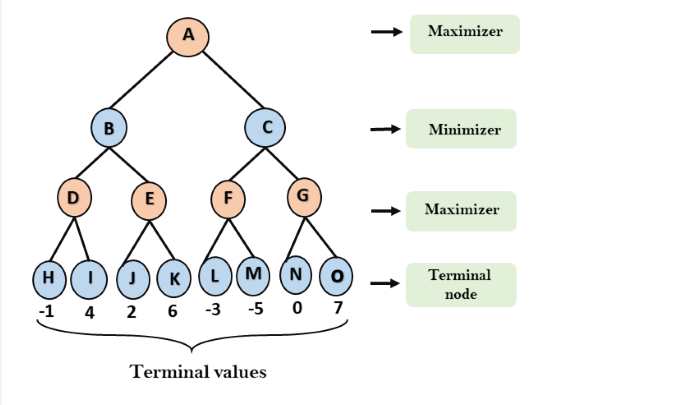
\includegraphics[width=\textwidth]{images/minimax.png}
\label{minimax}
\end{figure}
\subsubsection{Alpha-beta Pruning}
 could be described as an algorithm which aims to minimize the number of nodes that are given by the minimax in its search tree. It contains two values within the recursive functions which are named Alpha and Beta. Moreover, it is mostly used for 2 player machine games. To elaborate, the primary purpose of its use is to reduce the pruning of the search tree. Thus, it could be described as a modified version of the minimax algorithm, which is more optimal. Without that, applying alpha-beta pruning is always the most optimal approach to the task. Alpha-beta is considered faster than minimax because it does not explore some branches of the tree, which will not affect the value\footnote{Slagle, J. R 1963}. Thus, it will look twice as far in comparison to minimax in the same period of time.
\begin{figure}
\centering
\hspace*{-20pt}
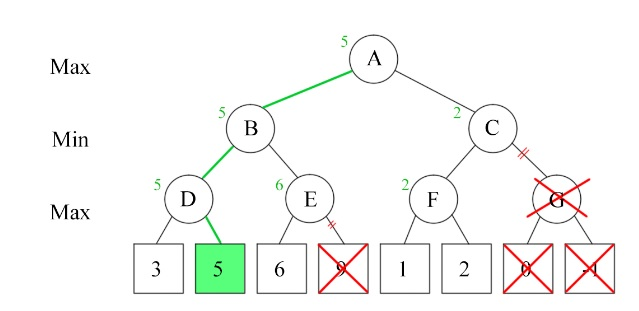
\includegraphics[width=\textwidth]{images/alphabeta.png}
\label{alphabeta}
\end{figure}
\subsubsection{Machine Learning}
(ML) is a branch of computer science intent on developing algorithms that can automatically learn from the input data. It generates algorithms that can learn a specific task without being programmed explicitly for it. It is mostly used for classification, regression, and clustering tasks\footnote{M. G. Bobra and S. Couvidat (2015)}. To elaborate, an ML bot would aim to “learn” by identifying new patterns through the data given in a process and create new strategies to improve the performance of a specific task and lead to the desired results\footnote{Karlijn, Willems (2018)}. Machine learning algorithms are used in an increasing amount of different tasks such as email filtering, image processing and game theory (poker, schnapsen, chess). In schnapsen, Machine learning bot can learn the heuristic function rather than implementing. The advantage of machine learning is that in schnapsen, is needed only to calculate one heuristic function. \\
In our research, we are using altering vectors of machine learning to achieve our goal. Vector machine is a supervised algorithm that is used for classification or regression problems where the dataset teaches SVM about the classes so that it can classify all new data. It works by arranging the information into various classes by finding a line (hyperplane) which isolates the data set into classes. This algorithm aims to maximize the distance between several different classes that are involved and is referred to as margin maximization. If the line that maximizes the distance between the classes is identified, the probability to generalize well to unseen data is increased. \\

\noindent There are four machine learning bots:
\begin{enumerate}
\item ml \textemdash \ this is the default bot that has the default features: the default features player’s 1 points, player’s 2 points, player’s 1 pending points, player’s 2 pending points, trump suit, phase of the game, the size of the stock, leader, whose turn and card played by an opponent
\item ml\_limited\footnote{Detailed practical code implementation can be found in Appendix B} \textemdash \ the additional bot with a reduced feature vector, including the features such as perspective, player’s 1 and 2 points, player’s 1 and 2 pending points
\item ml\_extended\footnote{Detailed practical code implementation can be found in Appendix A}  \textemdash \ the additional bot that consists of default features and features such as lowest card value for player, lowest card value for the opponent (phase 2), ace count for the player, ace count for opponent (phase 2), hand strength for player (number of points/max possible points), hand strength for opponent (number of points/max possible points, phase2), number of cards of opponent's suit in player's hand, point difference, pending point difference
\item ml\_mix\footnote{Detailed practical code implementation can be found in both Appendix A and B}  \textemdash \ the additional bot that consists of the feature vector, combined from ml\_limited and ml\_extended
\end{enumerate}
\end{document}